% Figura del nodo: metodo attuale (§9.1 / §7.1), versione del 20/11/2026. Compilare con: pdflatex nodi_new.tex
\documentclass[border=8pt]{standalone}
\usepackage[utf8]{inputenc}
\usepackage[T1]{fontenc}
\usepackage{lmodern}
\usepackage{amsmath,amssymb}
\usepackage{tikz}
\usetikzlibrary{arrows.meta,calc}
\renewcommand{\familydefault}{\sfdefault}
\definecolor{bl}{HTML}{2F6FD6}\definecolor{blf}{HTML}{DCE8FA}
\definecolor{orc}{HTML}{E8692B}\definecolor{orf}{HTML}{FBE3D6}
\definecolor{gr}{HTML}{9A9A9A}\definecolor{mid}{HTML}{666666}
\tikzset{
  dim/.style={{Latex[length=1.6mm]}-{Latex[length=1.6mm]},mid,thin},
  dimb/.style={{Latex[length=1.6mm]}-{Latex[length=1.6mm]},bl,semithick},
  dimo/.style={{Latex[length=1.6mm]}-{Latex[length=1.6mm]},orc,semithick},
  bfrect/.style={draw=bl,line width=1.1pt,fill=blf},
  flrect/.style={draw=orc,line width=1.1pt,fill=orf},
  prof/.style={gr,line width=1pt},
  ttl/.style={anchor=west,font=\bfseries\small},
  lab/.style={font=\footnotesize},
  note/.style={font=\scriptsize,text=mid},
}
\begin{document}
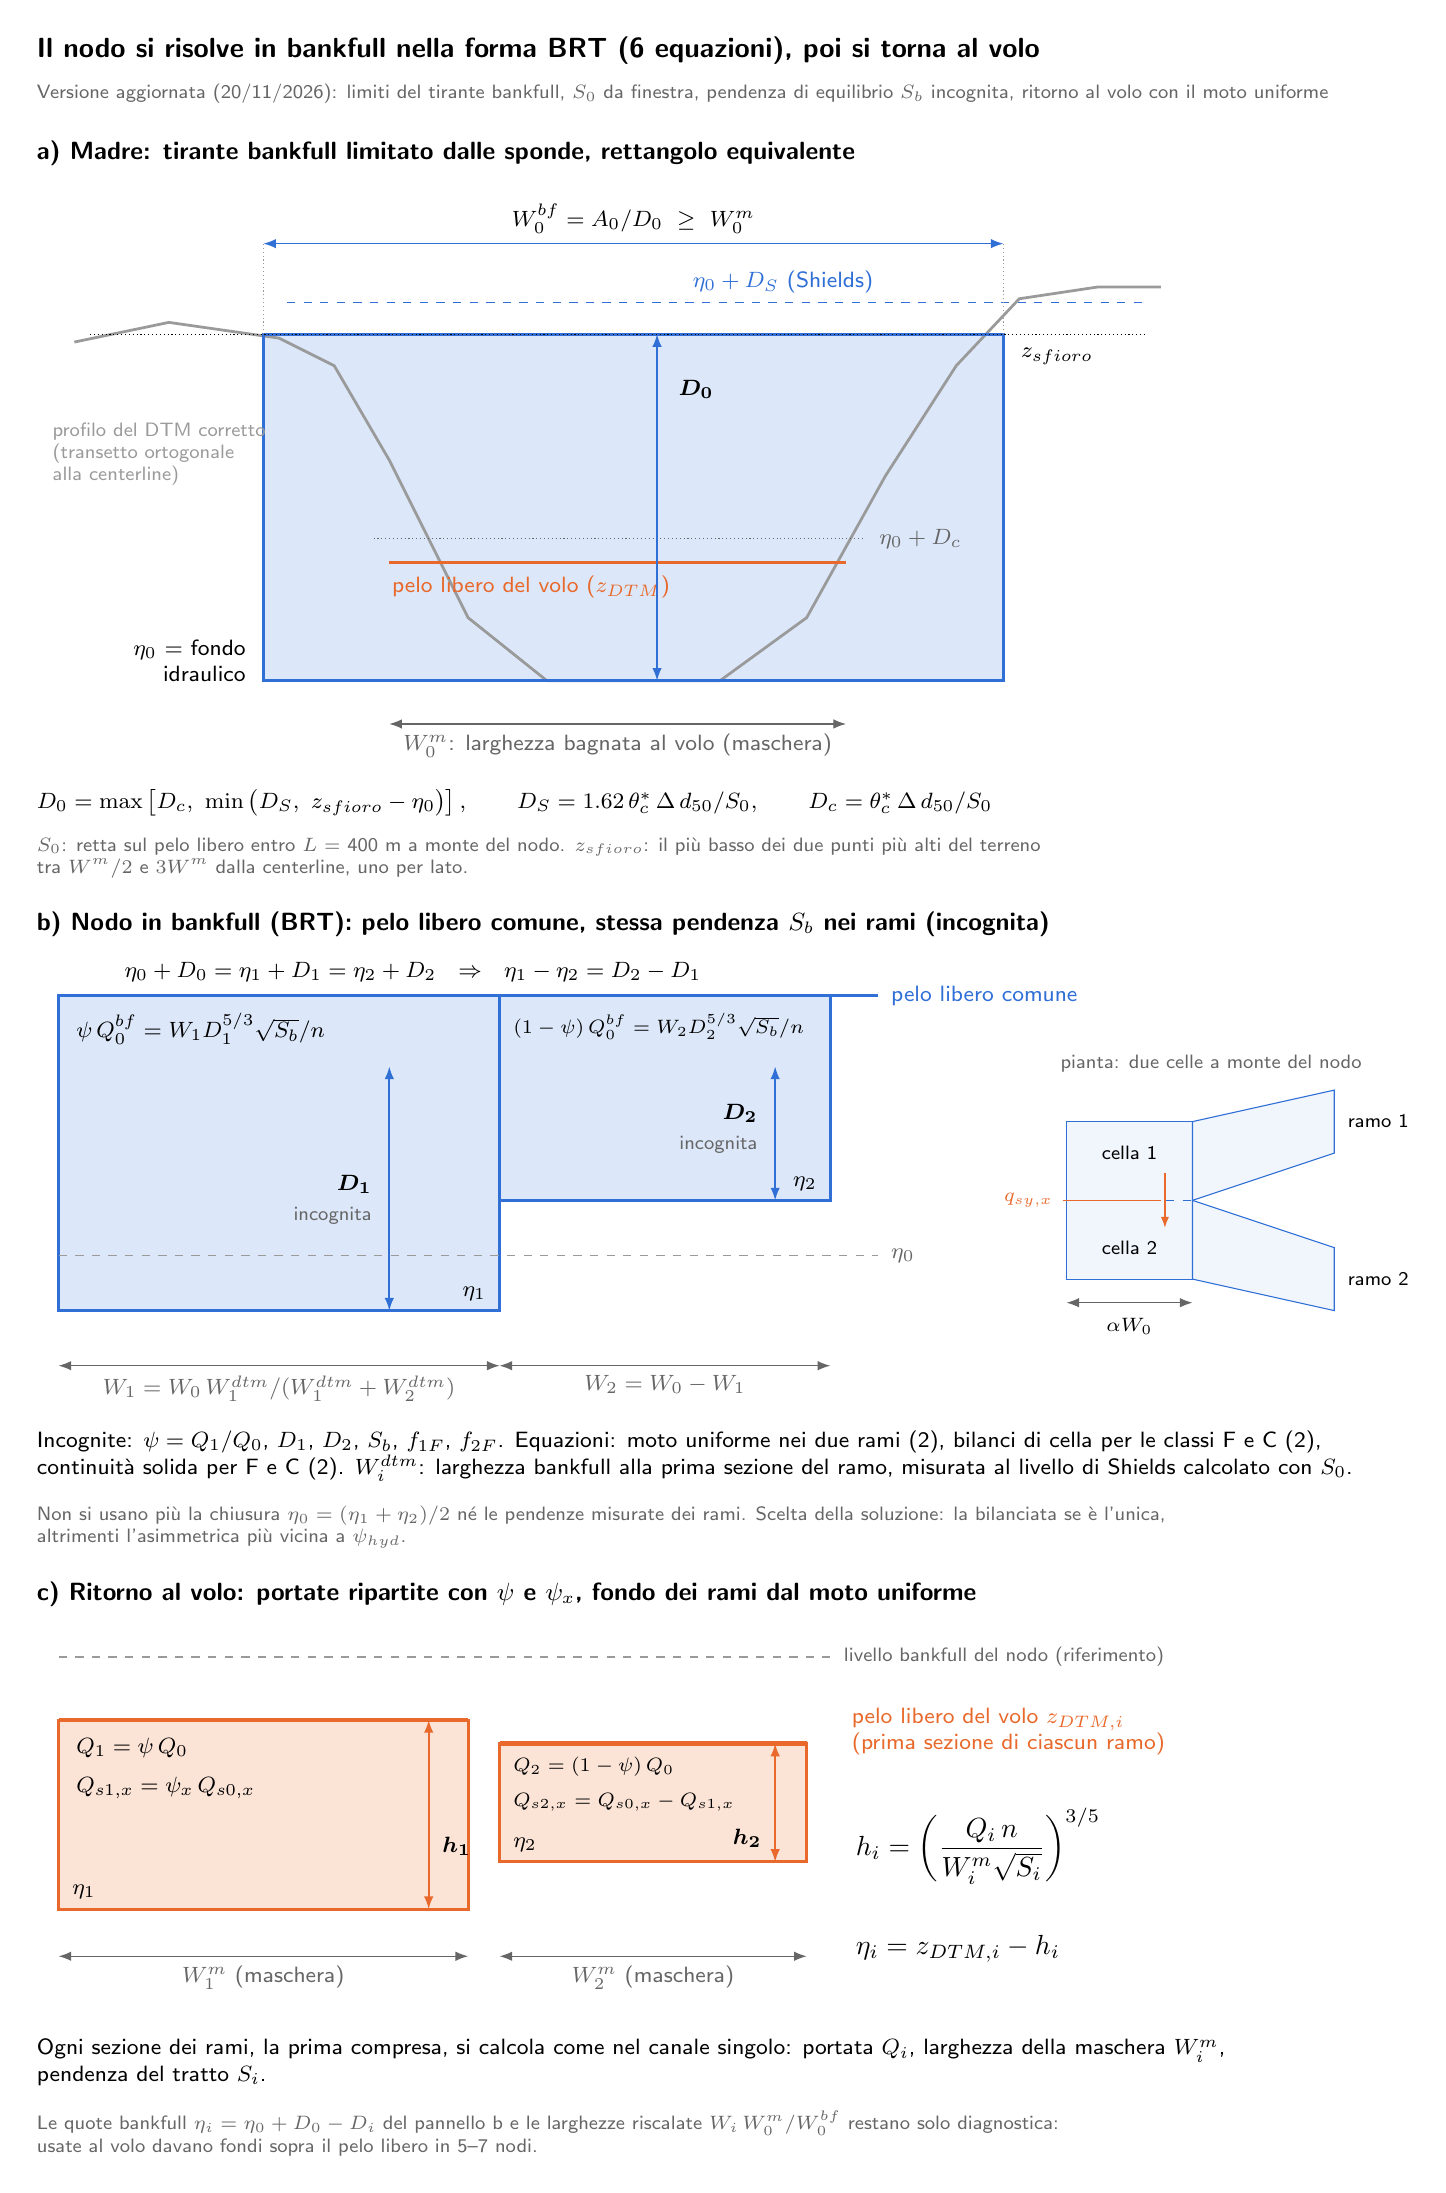
\begin{tikzpicture}[x=1cm,y=1cm]
\node[anchor=west,font=\bfseries\normalsize] at (0,0.6) {Il nodo si risolve in bankfull nella forma BRT (6 equazioni), poi si torna al volo};
\node[anchor=west,note] at (0,0.05) {Versione aggiornata (20/11/2026): limiti del tirante bankfull, $S_0$ da finestra, pendenza di equilibrio $S_b$ incognita, ritorno al volo con il moto uniforme};
% ---------------- a ----------------
\node[ttl] at (0,-0.7) {a) Madre: tirante bankfull limitato dalle sponde, rettangolo equivalente};
\begin{scope}[shift={(0,-7.6)}]
\fill[blf] (3.0,0.2) rectangle (12.4,4.6);
\draw[prof] (0.6,4.5) -- (1.8,4.75) -- (3.2,4.55) -- (3.9,4.2) -- (4.6,3.0) -- (5.6,1.0) -- (6.6,0.2) -- (8.8,0.2) -- (9.9,1.0) -- (10.9,2.8) -- (11.8,4.2) -- (12.6,5.05) -- (13.6,5.2) -- (14.4,5.2);
\draw[bl,line width=1.1pt] (3.0,0.2) rectangle (12.4,4.6);
\node[note,text=gr,anchor=north west,align=left] at (0.2,3.6) {profilo del DTM corretto\\(transetto ortogonale\\alla centerline)};
\draw[bl,dashed] (3.3,5.0) -- (14.2,5.0); \node[lab,text=bl,anchor=south] at (9.6,5.0) {$\eta_0+D_S$ (Shields)};
\draw[densely dotted] (0.8,4.6) -- (14.2,4.6); \node[lab,anchor=north west] at (12.5,4.55) {$z_{sfioro}$};
\draw[mid,densely dotted] (4.4,2.0) -- (10.6,2.0); \node[lab,text=mid,anchor=west] at (10.7,2.0) {$\eta_0+D_c$};
\draw[orc,line width=1.3pt] (4.6,1.7) -- (10.4,1.7); \node[lab,text=orc,anchor=north] at (6.4,1.65) {pelo libero del volo ($z_{DTM}$)};
\draw[dimb] (8.0,0.2) -- (8.0,4.6); \node[lab,anchor=west] at (8.15,3.9) {$\boldsymbol{D_0}$};
\node[lab,anchor=east,align=right] at (2.9,0.45) {$\eta_0$ = fondo\\idraulico};
\draw[dimb] (3.0,5.75) -- (12.4,5.75) node[midway,above,lab,text=black] {$W_0^{bf}=A_0/D_0\ \geq\ W_0^{m}$};
\draw[gr,densely dotted] (3.0,4.6) -- (3.0,5.75); \draw[gr,densely dotted] (12.4,4.6) -- (12.4,5.75);
\draw[dim] (4.6,-0.35) -- (10.4,-0.35) node[midway,below,lab] {$W_0^{m}$: larghezza bagnata al volo (maschera)};
\node[lab,anchor=west] at (0,-1.35) {$D_0=\max\left[D_c,\ \min\left(D_S,\ z_{sfioro}-\eta_0\right)\right],\qquad D_S=1.62\,\theta^{*}_c\,\Delta\,d_{50}/S_0,\qquad D_c=\theta^{*}_c\,\Delta\,d_{50}/S_0$};
\node[note,anchor=west,align=left] at (0,-2.05) {$S_0$: retta sul pelo libero entro $L$ = 400 m a monte del nodo. $z_{sfioro}$: il più basso dei due punti più alti del terreno\\tra $W^m/2$ e $3W^m$ dalla centerline, uno per lato.};
\end{scope}
% ---------------- b ----------------
\node[ttl] at (0,-10.5) {b) Nodo in bankfull (BRT): pelo libero comune, stessa pendenza $S_b$ nei rami (incognita)};
\begin{scope}[shift={(0,-16.0)}]
\node[lab,anchor=south] at (4.9,4.65) {$\eta_0+D_0=\eta_1+D_1=\eta_2+D_2\ \ \Rightarrow\ \ \eta_1-\eta_2=D_2-D_1$};
\draw[bfrect] (0.4,0.6) rectangle (6.0,4.6);
\draw[bfrect] (6.0,2.0) rectangle (10.2,4.6);
\draw[bl,line width=1pt] (0.4,4.6) -- (10.8,4.6); \node[lab,text=bl,anchor=west] at (10.85,4.6) {pelo libero comune};
\draw[gr,dashed] (0.4,1.3) -- (10.8,1.3); \node[lab,text=mid,anchor=west] at (10.85,1.3) {$\eta_0$};
\node[lab,anchor=north west] at (0.5,4.5) {$\psi\,Q_0^{bf}=W_1D_1^{5/3}\sqrt{S_b}/n$};
\node[lab,anchor=north west,font=\scriptsize] at (6.05,4.5) {$(1-\psi)\,Q_0^{bf}=W_2D_2^{5/3}\sqrt{S_b}/n$};
\draw[dimb] (4.6,0.6) -- (4.6,3.7); \node[lab,anchor=east] at (4.5,2.2) {$\boldsymbol{D_1}$}; \node[note,anchor=east] at (4.5,1.8) {incognita};
\draw[dimb] (9.5,2.0) -- (9.5,3.7); \node[lab,anchor=east] at (9.4,3.1) {$\boldsymbol{D_2}$}; \node[note,anchor=east] at (9.4,2.7) {incognita};
\node[lab,anchor=south east] at (5.95,0.6) {$\eta_1$}; \node[lab,anchor=south east] at (10.15,2.0) {$\eta_2$};
\draw[dim] (0.4,-0.1) -- (6.0,-0.1) node[midway,below,lab] {$W_1=W_0\,W_1^{dtm}/(W_1^{dtm}+W_2^{dtm})$};
\draw[dim] (6.0,-0.1) -- (10.2,-0.1) node[midway,below,lab] {$W_2=W_0-W_1$};
% planform
\begin{scope}[shift={(13.2,0.4)}]
\node[note,anchor=south west] at (-0.2,3.1) {pianta: due celle a monte del nodo};
\draw[bl,fill=blf!40] (0,0.6) rectangle (1.6,2.6);
\draw[bl,dashed,thin] (0,1.6) -- (1.6,1.6);
\draw[bl,fill=blf!40] (1.6,2.6) -- (3.4,3.0) -- (3.4,2.2) -- (1.6,1.6) -- cycle;
\draw[bl,fill=blf!40] (1.6,1.6) -- (3.4,1.0) -- (3.4,0.2) -- (1.6,0.6) -- cycle;
\node[note,text=black] at (0.8,2.2) {cella 1}; \node[note,text=black] at (0.8,1.0) {cella 2};
\draw[-{Latex[length=1.4mm]},orc,semithick] (1.25,1.95) -- (1.25,1.25); \node[note,text=orc,anchor=east] at (-0.05,1.6) {$q_{sy,x}$}; \draw[orc,thin] (-0.05,1.6) -- (1.2,1.6);
\node[note,text=black,anchor=west] at (3.45,2.6) {ramo 1}; \node[note,text=black,anchor=west] at (3.45,0.6) {ramo 2};
\draw[dim] (0,0.3) -- (1.6,0.3); \node[note,text=black] at (0.8,0.0) {$\alpha W_0$};
\end{scope}
\node[lab,anchor=west,align=left] at (0,-1.25) {Incognite: $\psi=Q_1/Q_0$, $D_1$, $D_2$, $S_b$, $f_{1F}$, $f_{2F}$. Equazioni: moto uniforme nei due rami (2), bilanci di cella per le classi F e C (2),\\continuità solida per F e C (2). $W_i^{dtm}$: larghezza bankfull alla prima sezione del ramo, misurata al livello di Shields calcolato con $S_0$.};
\node[note,anchor=west,align=left] at (0,-2.15) {Non si usano più la chiusura $\eta_0=(\eta_1+\eta_2)/2$ né le pendenze misurate dei rami. Scelta della soluzione: la bilanciata se è l'unica,\\altrimenti l'asimmetrica più vicina a $\psi_{hyd}$.};
\end{scope}
% ---------------- c ----------------
\node[ttl] at (0,-19.0) {c) Ritorno al volo: portate ripartite con $\psi$ e $\psi_x$, fondo dei rami dal moto uniforme};
\begin{scope}[shift={(0,-24.2)}]
\draw[gr,dashed] (0.4,4.4) -- (10.2,4.4); \node[note,anchor=west] at (10.25,4.4) {livello bankfull del nodo (riferimento)};
\draw[flrect] (0.4,1.2) rectangle (5.6,3.6);
\draw[flrect] (6.0,1.8) rectangle (9.9,3.3);
\draw[orc,line width=1.6pt] (0.4,3.6) -- (5.6,3.6); \draw[orc,line width=1.6pt] (6.0,3.3) -- (9.9,3.3);
\node[lab,text=orc,anchor=west,align=left] at (10.35,3.45) {pelo libero del volo $z_{DTM,i}$\\(prima sezione di ciascun ramo)};
\node[lab,anchor=north west] at (0.5,3.5) {$Q_1=\psi\,Q_0$}; \node[lab,anchor=north west] at (0.5,3.0) {$Q_{s1,x}=\psi_x\,Q_{s0,x}$};
\node[lab,anchor=north west,font=\scriptsize] at (6.05,3.25) {$Q_2=(1-\psi)\,Q_0$}; \node[lab,anchor=north west,font=\scriptsize] at (6.05,2.8) {$Q_{s2,x}=Q_{s0,x}-Q_{s1,x}$};
\draw[dimo] (5.1,1.2) -- (5.1,3.6); \node[lab,anchor=west] at (5.15,2.0) {$\boldsymbol{h_1}$};
\draw[dimo] (9.5,1.8) -- (9.5,3.3); \node[lab,anchor=east] at (9.45,2.1) {$\boldsymbol{h_2}$};
\node[lab,anchor=south west] at (0.45,1.2) {$\eta_1$}; \node[lab,anchor=south west] at (6.05,1.8) {$\eta_2$};
\draw[dim] (0.4,0.6) -- (5.6,0.6) node[midway,below,lab] {$W_1^{m}$ (maschera)};
\draw[dim] (6.0,0.6) -- (9.9,0.6) node[midway,below,lab] {$W_2^{m}$ (maschera)};
\node[anchor=west] at (10.4,2.0) {$\displaystyle h_i=\left(\frac{Q_i\,n}{W_i^{m}\sqrt{S_i}}\right)^{3/5}$};
\node[anchor=west] at (10.4,0.7) {$\eta_i=z_{DTM,i}-h_i$};
\node[lab,anchor=west,align=left] at (0,-0.75) {Ogni sezione dei rami, la prima compresa, si calcola come nel canale singolo: portata $Q_i$, larghezza della maschera $W_i^m$,\\pendenza del tratto $S_i$.};
\node[note,anchor=west,align=left] at (0,-1.65) {Le quote bankfull $\eta_i=\eta_0+D_0-D_i$ del pannello b e le larghezze riscalate $W_i\,W_0^m/W_0^{bf}$ restano solo diagnostica:\\usate al volo davano fondi sopra il pelo libero in 5--7 nodi.};
\end{scope}
\end{tikzpicture}
\end{document}
